% Created by tikzDevice version 0.10.1 on 2016-08-26 09:57:47
% !TEX encoding = UTF-8 Unicode
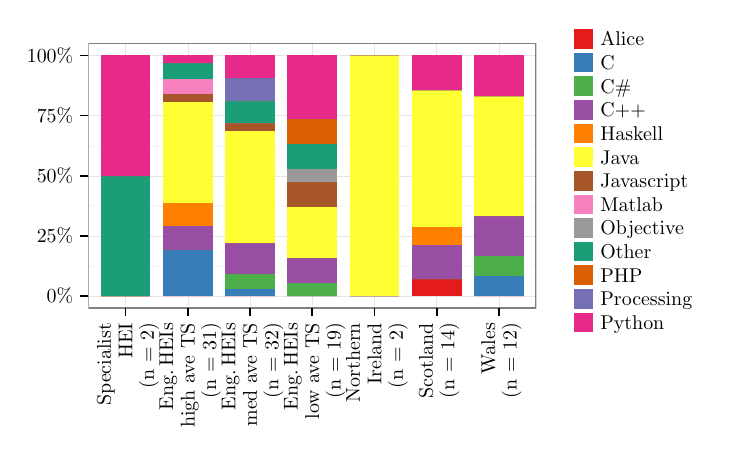
\begin{tikzpicture}[x=1pt,y=1pt]
\definecolor{fillColor}{RGB}{255,255,255}
\path[use as bounding box,fill=fillColor,fill opacity=0.00] (0,0) rectangle (252.94,144.54);
\begin{scope}
\path[clip] (  0.00,  0.00) rectangle (252.94,144.54);
\definecolor{drawColor}{RGB}{255,255,255}
\definecolor{fillColor}{RGB}{255,255,255}

\path[draw=drawColor,line width= 0.6pt,line join=round,line cap=round,fill=fillColor] (  0.00,  0.00) rectangle (252.94,144.54);
\end{scope}
\begin{scope}
\path[clip] ( 21.89, 43.19) rectangle (183.80,138.85);
\definecolor{fillColor}{RGB}{255,255,255}

\path[fill=fillColor] ( 21.89, 43.19) rectangle (183.80,138.85);
\definecolor{drawColor}{gray}{0.98}

\path[draw=drawColor,line width= 0.6pt,line join=round] ( 21.89, 58.41) --
	(183.80, 58.41);

\path[draw=drawColor,line width= 0.6pt,line join=round] ( 21.89, 80.15) --
	(183.80, 80.15);

\path[draw=drawColor,line width= 0.6pt,line join=round] ( 21.89,101.89) --
	(183.80,101.89);

\path[draw=drawColor,line width= 0.6pt,line join=round] ( 21.89,123.63) --
	(183.80,123.63);
\definecolor{drawColor}{gray}{0.90}

\path[draw=drawColor,line width= 0.2pt,line join=round] ( 21.89, 47.54) --
	(183.80, 47.54);

\path[draw=drawColor,line width= 0.2pt,line join=round] ( 21.89, 69.28) --
	(183.80, 69.28);

\path[draw=drawColor,line width= 0.2pt,line join=round] ( 21.89, 91.02) --
	(183.80, 91.02);

\path[draw=drawColor,line width= 0.2pt,line join=round] ( 21.89,112.76) --
	(183.80,112.76);

\path[draw=drawColor,line width= 0.2pt,line join=round] ( 21.89,134.50) --
	(183.80,134.50);

\path[draw=drawColor,line width= 0.2pt,line join=round] ( 35.38, 43.19) --
	( 35.38,138.85);

\path[draw=drawColor,line width= 0.2pt,line join=round] ( 57.87, 43.19) --
	( 57.87,138.85);

\path[draw=drawColor,line width= 0.2pt,line join=round] ( 80.36, 43.19) --
	( 80.36,138.85);

\path[draw=drawColor,line width= 0.2pt,line join=round] (102.85, 43.19) --
	(102.85,138.85);

\path[draw=drawColor,line width= 0.2pt,line join=round] (125.33, 43.19) --
	(125.33,138.85);

\path[draw=drawColor,line width= 0.2pt,line join=round] (147.82, 43.19) --
	(147.82,138.85);

\path[draw=drawColor,line width= 0.2pt,line join=round] (170.31, 43.19) --
	(170.31,138.85);
\definecolor{fillColor}{RGB}{228,26,28}

\path[fill=fillColor] ( 26.39, 47.54) rectangle ( 44.38, 47.54);
\definecolor{fillColor}{RGB}{55,126,184}

\path[fill=fillColor] ( 26.39, 47.54) rectangle ( 44.38, 47.54);
\definecolor{fillColor}{RGB}{77,175,74}

\path[fill=fillColor] ( 26.39, 47.54) rectangle ( 44.38, 47.54);
\definecolor{fillColor}{RGB}{152,78,163}

\path[fill=fillColor] ( 26.39, 47.54) rectangle ( 44.38, 47.54);
\definecolor{fillColor}{RGB}{255,127,0}

\path[fill=fillColor] ( 26.39, 47.54) rectangle ( 44.38, 47.54);
\definecolor{fillColor}{RGB}{255,255,51}

\path[fill=fillColor] ( 26.39, 47.54) rectangle ( 44.38, 47.54);
\definecolor{fillColor}{RGB}{166,86,40}

\path[fill=fillColor] ( 26.39, 47.54) rectangle ( 44.38, 47.54);
\definecolor{fillColor}{RGB}{247,129,191}

\path[fill=fillColor] ( 26.39, 47.54) rectangle ( 44.38, 47.54);
\definecolor{fillColor}{gray}{0.60}

\path[fill=fillColor] ( 26.39, 47.54) rectangle ( 44.38, 47.54);
\definecolor{fillColor}{RGB}{27,158,119}

\path[fill=fillColor] ( 26.39, 47.54) rectangle ( 44.38, 91.02);
\definecolor{fillColor}{RGB}{217,95,2}

\path[fill=fillColor] ( 26.39, 91.02) rectangle ( 44.38, 91.02);
\definecolor{fillColor}{RGB}{117,112,179}

\path[fill=fillColor] ( 26.39, 91.02) rectangle ( 44.38, 91.02);
\definecolor{fillColor}{RGB}{231,41,138}

\path[fill=fillColor] ( 26.39, 91.02) rectangle ( 44.38,134.50);
\definecolor{fillColor}{RGB}{228,26,28}

\path[fill=fillColor] ( 48.87, 47.54) rectangle ( 66.86, 47.54);
\definecolor{fillColor}{RGB}{55,126,184}

\path[fill=fillColor] ( 48.87, 47.54) rectangle ( 66.86, 64.37);
\definecolor{fillColor}{RGB}{77,175,74}

\path[fill=fillColor] ( 48.87, 64.37) rectangle ( 66.86, 64.37);
\definecolor{fillColor}{RGB}{152,78,163}

\path[fill=fillColor] ( 48.87, 64.37) rectangle ( 66.86, 72.79);
\definecolor{fillColor}{RGB}{255,127,0}

\path[fill=fillColor] ( 48.87, 72.79) rectangle ( 66.86, 81.20);
\definecolor{fillColor}{RGB}{255,255,51}

\path[fill=fillColor] ( 48.87, 81.20) rectangle ( 66.86,117.67);
\definecolor{fillColor}{RGB}{166,86,40}

\path[fill=fillColor] ( 48.87,117.67) rectangle ( 66.86,120.48);
\definecolor{fillColor}{RGB}{247,129,191}

\path[fill=fillColor] ( 48.87,120.48) rectangle ( 66.86,126.09);
\definecolor{fillColor}{gray}{0.60}

\path[fill=fillColor] ( 48.87,126.09) rectangle ( 66.86,126.09);
\definecolor{fillColor}{RGB}{27,158,119}

\path[fill=fillColor] ( 48.87,126.09) rectangle ( 66.86,131.70);
\definecolor{fillColor}{RGB}{217,95,2}

\path[fill=fillColor] ( 48.87,131.70) rectangle ( 66.86,131.70);
\definecolor{fillColor}{RGB}{117,112,179}

\path[fill=fillColor] ( 48.87,131.70) rectangle ( 66.86,131.70);
\definecolor{fillColor}{RGB}{231,41,138}

\path[fill=fillColor] ( 48.87,131.70) rectangle ( 66.86,134.50);
\definecolor{fillColor}{RGB}{228,26,28}

\path[fill=fillColor] ( 71.36, 47.54) rectangle ( 89.35, 47.54);
\definecolor{fillColor}{RGB}{55,126,184}

\path[fill=fillColor] ( 71.36, 47.54) rectangle ( 89.35, 50.26);
\definecolor{fillColor}{RGB}{77,175,74}

\path[fill=fillColor] ( 71.36, 50.26) rectangle ( 89.35, 55.69);
\definecolor{fillColor}{RGB}{152,78,163}

\path[fill=fillColor] ( 71.36, 55.69) rectangle ( 89.35, 66.56);
\definecolor{fillColor}{RGB}{255,127,0}

\path[fill=fillColor] ( 71.36, 66.56) rectangle ( 89.35, 66.56);
\definecolor{fillColor}{RGB}{255,255,51}

\path[fill=fillColor] ( 71.36, 66.56) rectangle ( 89.35,107.33);
\definecolor{fillColor}{RGB}{166,86,40}

\path[fill=fillColor] ( 71.36,107.33) rectangle ( 89.35,110.04);
\definecolor{fillColor}{RGB}{247,129,191}

\path[fill=fillColor] ( 71.36,110.04) rectangle ( 89.35,110.04);
\definecolor{fillColor}{gray}{0.60}

\path[fill=fillColor] ( 71.36,110.04) rectangle ( 89.35,110.04);
\definecolor{fillColor}{RGB}{27,158,119}

\path[fill=fillColor] ( 71.36,110.04) rectangle ( 89.35,118.20);
\definecolor{fillColor}{RGB}{217,95,2}

\path[fill=fillColor] ( 71.36,118.20) rectangle ( 89.35,118.20);
\definecolor{fillColor}{RGB}{117,112,179}

\path[fill=fillColor] ( 71.36,118.20) rectangle ( 89.35,126.35);
\definecolor{fillColor}{RGB}{231,41,138}

\path[fill=fillColor] ( 71.36,126.35) rectangle ( 89.35,134.50);
\definecolor{fillColor}{RGB}{228,26,28}

\path[fill=fillColor] ( 93.85, 47.54) rectangle (111.84, 47.54);
\definecolor{fillColor}{RGB}{55,126,184}

\path[fill=fillColor] ( 93.85, 47.54) rectangle (111.84, 47.54);
\definecolor{fillColor}{RGB}{77,175,74}

\path[fill=fillColor] ( 93.85, 47.54) rectangle (111.84, 52.12);
\definecolor{fillColor}{RGB}{152,78,163}

\path[fill=fillColor] ( 93.85, 52.12) rectangle (111.84, 61.27);
\definecolor{fillColor}{RGB}{255,127,0}

\path[fill=fillColor] ( 93.85, 61.27) rectangle (111.84, 61.27);
\definecolor{fillColor}{RGB}{255,255,51}

\path[fill=fillColor] ( 93.85, 61.27) rectangle (111.84, 79.58);
\definecolor{fillColor}{RGB}{166,86,40}

\path[fill=fillColor] ( 93.85, 79.58) rectangle (111.84, 88.73);
\definecolor{fillColor}{RGB}{247,129,191}

\path[fill=fillColor] ( 93.85, 88.73) rectangle (111.84, 88.73);
\definecolor{fillColor}{gray}{0.60}

\path[fill=fillColor] ( 93.85, 88.73) rectangle (111.84, 93.31);
\definecolor{fillColor}{RGB}{27,158,119}

\path[fill=fillColor] ( 93.85, 93.31) rectangle (111.84,102.46);
\definecolor{fillColor}{RGB}{217,95,2}

\path[fill=fillColor] ( 93.85,102.46) rectangle (111.84,111.62);
\definecolor{fillColor}{RGB}{117,112,179}

\path[fill=fillColor] ( 93.85,111.62) rectangle (111.84,111.62);
\definecolor{fillColor}{RGB}{231,41,138}

\path[fill=fillColor] ( 93.85,111.62) rectangle (111.84,134.50);
\definecolor{fillColor}{RGB}{228,26,28}

\path[fill=fillColor] (116.34, 47.54) rectangle (134.33, 47.54);
\definecolor{fillColor}{RGB}{55,126,184}

\path[fill=fillColor] (116.34, 47.54) rectangle (134.33, 47.54);
\definecolor{fillColor}{RGB}{77,175,74}

\path[fill=fillColor] (116.34, 47.54) rectangle (134.33, 47.54);
\definecolor{fillColor}{RGB}{152,78,163}

\path[fill=fillColor] (116.34, 47.54) rectangle (134.33, 47.54);
\definecolor{fillColor}{RGB}{255,127,0}

\path[fill=fillColor] (116.34, 47.54) rectangle (134.33, 47.54);
\definecolor{fillColor}{RGB}{255,255,51}

\path[fill=fillColor] (116.34, 47.54) rectangle (134.33,134.50);
\definecolor{fillColor}{RGB}{166,86,40}

\path[fill=fillColor] (116.34,134.50) rectangle (134.33,134.50);
\definecolor{fillColor}{RGB}{247,129,191}

\path[fill=fillColor] (116.34,134.50) rectangle (134.33,134.50);
\definecolor{fillColor}{gray}{0.60}

\path[fill=fillColor] (116.34,134.50) rectangle (134.33,134.50);
\definecolor{fillColor}{RGB}{27,158,119}

\path[fill=fillColor] (116.34,134.50) rectangle (134.33,134.50);
\definecolor{fillColor}{RGB}{217,95,2}

\path[fill=fillColor] (116.34,134.50) rectangle (134.33,134.50);
\definecolor{fillColor}{RGB}{117,112,179}

\path[fill=fillColor] (116.34,134.50) rectangle (134.33,134.50);
\definecolor{fillColor}{RGB}{231,41,138}

\path[fill=fillColor] (116.34,134.50) rectangle (134.33,134.50);
\definecolor{fillColor}{RGB}{228,26,28}

\path[fill=fillColor] (138.83, 47.54) rectangle (156.82, 53.75);
\definecolor{fillColor}{RGB}{55,126,184}

\path[fill=fillColor] (138.83, 53.75) rectangle (156.82, 53.75);
\definecolor{fillColor}{RGB}{77,175,74}

\path[fill=fillColor] (138.83, 53.75) rectangle (156.82, 53.75);
\definecolor{fillColor}{RGB}{152,78,163}

\path[fill=fillColor] (138.83, 53.75) rectangle (156.82, 66.17);
\definecolor{fillColor}{RGB}{255,127,0}

\path[fill=fillColor] (138.83, 66.17) rectangle (156.82, 72.39);
\definecolor{fillColor}{RGB}{255,255,51}

\path[fill=fillColor] (138.83, 72.39) rectangle (156.82,122.08);
\definecolor{fillColor}{RGB}{166,86,40}

\path[fill=fillColor] (138.83,122.08) rectangle (156.82,122.08);
\definecolor{fillColor}{RGB}{247,129,191}

\path[fill=fillColor] (138.83,122.08) rectangle (156.82,122.08);
\definecolor{fillColor}{gray}{0.60}

\path[fill=fillColor] (138.83,122.08) rectangle (156.82,122.08);
\definecolor{fillColor}{RGB}{27,158,119}

\path[fill=fillColor] (138.83,122.08) rectangle (156.82,122.08);
\definecolor{fillColor}{RGB}{217,95,2}

\path[fill=fillColor] (138.83,122.08) rectangle (156.82,122.08);
\definecolor{fillColor}{RGB}{117,112,179}

\path[fill=fillColor] (138.83,122.08) rectangle (156.82,122.08);
\definecolor{fillColor}{RGB}{231,41,138}

\path[fill=fillColor] (138.83,122.08) rectangle (156.82,134.50);
\definecolor{fillColor}{RGB}{228,26,28}

\path[fill=fillColor] (161.31, 47.54) rectangle (179.31, 47.54);
\definecolor{fillColor}{RGB}{55,126,184}

\path[fill=fillColor] (161.31, 47.54) rectangle (179.31, 54.79);
\definecolor{fillColor}{RGB}{77,175,74}

\path[fill=fillColor] (161.31, 54.79) rectangle (179.31, 62.03);
\definecolor{fillColor}{RGB}{152,78,163}

\path[fill=fillColor] (161.31, 62.03) rectangle (179.31, 76.53);
\definecolor{fillColor}{RGB}{255,127,0}

\path[fill=fillColor] (161.31, 76.53) rectangle (179.31, 76.53);
\definecolor{fillColor}{RGB}{255,255,51}

\path[fill=fillColor] (161.31, 76.53) rectangle (179.31,120.01);
\definecolor{fillColor}{RGB}{166,86,40}

\path[fill=fillColor] (161.31,120.01) rectangle (179.31,120.01);
\definecolor{fillColor}{RGB}{247,129,191}

\path[fill=fillColor] (161.31,120.01) rectangle (179.31,120.01);
\definecolor{fillColor}{gray}{0.60}

\path[fill=fillColor] (161.31,120.01) rectangle (179.31,120.01);
\definecolor{fillColor}{RGB}{27,158,119}

\path[fill=fillColor] (161.31,120.01) rectangle (179.31,120.01);
\definecolor{fillColor}{RGB}{217,95,2}

\path[fill=fillColor] (161.31,120.01) rectangle (179.31,120.01);
\definecolor{fillColor}{RGB}{117,112,179}

\path[fill=fillColor] (161.31,120.01) rectangle (179.31,120.01);
\definecolor{fillColor}{RGB}{231,41,138}

\path[fill=fillColor] (161.31,120.01) rectangle (179.31,134.50);
\definecolor{drawColor}{gray}{0.50}

\path[draw=drawColor,line width= 0.6pt,line join=round,line cap=round] ( 21.89, 43.19) rectangle (183.80,138.85);
\end{scope}
\begin{scope}
\path[clip] (  0.00,  0.00) rectangle (252.94,144.54);
\definecolor{drawColor}{RGB}{0,0,0}

\node[text=drawColor,anchor=base east,inner sep=0pt, outer sep=0pt, scale=  0.72] at ( 16.49, 45.06) {0\%};

\node[text=drawColor,anchor=base east,inner sep=0pt, outer sep=0pt, scale=  0.72] at ( 16.49, 66.80) {25\%};

\node[text=drawColor,anchor=base east,inner sep=0pt, outer sep=0pt, scale=  0.72] at ( 16.49, 88.54) {50\%};

\node[text=drawColor,anchor=base east,inner sep=0pt, outer sep=0pt, scale=  0.72] at ( 16.49,110.28) {75\%};

\node[text=drawColor,anchor=base east,inner sep=0pt, outer sep=0pt, scale=  0.72] at ( 16.49,132.02) {100\%};
\end{scope}
\begin{scope}
\path[clip] (  0.00,  0.00) rectangle (252.94,144.54);
\definecolor{drawColor}{RGB}{0,0,0}

\path[draw=drawColor,line width= 0.6pt,line join=round] ( 18.89, 47.54) --
	( 21.89, 47.54);

\path[draw=drawColor,line width= 0.6pt,line join=round] ( 18.89, 69.28) --
	( 21.89, 69.28);

\path[draw=drawColor,line width= 0.6pt,line join=round] ( 18.89, 91.02) --
	( 21.89, 91.02);

\path[draw=drawColor,line width= 0.6pt,line join=round] ( 18.89,112.76) --
	( 21.89,112.76);

\path[draw=drawColor,line width= 0.6pt,line join=round] ( 18.89,134.50) --
	( 21.89,134.50);
\end{scope}
\begin{scope}
\path[clip] (  0.00,  0.00) rectangle (252.94,144.54);
\definecolor{drawColor}{RGB}{0,0,0}

\path[draw=drawColor,line width= 0.6pt,line join=round] ( 35.38, 40.19) --
	( 35.38, 43.19);

\path[draw=drawColor,line width= 0.6pt,line join=round] ( 57.87, 40.19) --
	( 57.87, 43.19);

\path[draw=drawColor,line width= 0.6pt,line join=round] ( 80.36, 40.19) --
	( 80.36, 43.19);

\path[draw=drawColor,line width= 0.6pt,line join=round] (102.85, 40.19) --
	(102.85, 43.19);

\path[draw=drawColor,line width= 0.6pt,line join=round] (125.33, 40.19) --
	(125.33, 43.19);

\path[draw=drawColor,line width= 0.6pt,line join=round] (147.82, 40.19) --
	(147.82, 43.19);

\path[draw=drawColor,line width= 0.6pt,line join=round] (170.31, 40.19) --
	(170.31, 43.19);
\end{scope}
\begin{scope}
\path[clip] (  0.00,  0.00) rectangle (252.94,144.54);
\definecolor{drawColor}{RGB}{0,0,0}

\node[text=drawColor,rotate= 90.00,anchor=base east,inner sep=0pt, outer sep=0pt, scale=  0.72] at ( 30.08, 37.79) {Specialist};

\node[text=drawColor,rotate= 90.00,anchor=base east,inner sep=0pt, outer sep=0pt, scale=  0.72] at ( 37.86, 37.79) {HEI};

\node[text=drawColor,rotate= 90.00,anchor=base east,inner sep=0pt, outer sep=0pt, scale=  0.72] at ( 45.64, 37.79) {(n = 2)};

\node[text=drawColor,rotate= 90.00,anchor=base east,inner sep=0pt, outer sep=0pt, scale=  0.72] at ( 52.57, 37.79) {Eng.\,HEIs};

\node[text=drawColor,rotate= 90.00,anchor=base east,inner sep=0pt, outer sep=0pt, scale=  0.72] at ( 60.35, 37.79) {high ave TS};

\node[text=drawColor,rotate= 90.00,anchor=base east,inner sep=0pt, outer sep=0pt, scale=  0.72] at ( 68.12, 37.79) {(n = 31)};

\node[text=drawColor,rotate= 90.00,anchor=base east,inner sep=0pt, outer sep=0pt, scale=  0.72] at ( 75.06, 37.79) {Eng.\,HEIs};

\node[text=drawColor,rotate= 90.00,anchor=base east,inner sep=0pt, outer sep=0pt, scale=  0.72] at ( 82.84, 37.79) {med ave TS};

\node[text=drawColor,rotate= 90.00,anchor=base east,inner sep=0pt, outer sep=0pt, scale=  0.72] at ( 90.61, 37.79) {(n = 32)};

\node[text=drawColor,rotate= 90.00,anchor=base east,inner sep=0pt, outer sep=0pt, scale=  0.72] at ( 97.55, 37.79) {Eng.\,HEIs};

\node[text=drawColor,rotate= 90.00,anchor=base east,inner sep=0pt, outer sep=0pt, scale=  0.72] at (105.32, 37.79) {low ave TS};

\node[text=drawColor,rotate= 90.00,anchor=base east,inner sep=0pt, outer sep=0pt, scale=  0.72] at (113.10, 37.79) {(n = 19)};

\node[text=drawColor,rotate= 90.00,anchor=base east,inner sep=0pt, outer sep=0pt, scale=  0.72] at (120.04, 37.79) {Northern};

\node[text=drawColor,rotate= 90.00,anchor=base east,inner sep=0pt, outer sep=0pt, scale=  0.72] at (127.81, 37.79) {Ireland};

\node[text=drawColor,rotate= 90.00,anchor=base east,inner sep=0pt, outer sep=0pt, scale=  0.72] at (135.59, 37.79) {(n = 2)};

\node[text=drawColor,rotate= 90.00,anchor=base east,inner sep=0pt, outer sep=0pt, scale=  0.72] at (146.41, 37.79) {Scotland};

\node[text=drawColor,rotate= 90.00,anchor=base east,inner sep=0pt, outer sep=0pt, scale=  0.72] at (154.19, 37.79) {(n = 14)};

\node[text=drawColor,rotate= 90.00,anchor=base east,inner sep=0pt, outer sep=0pt, scale=  0.72] at (168.90, 37.79) {Wales};

\node[text=drawColor,rotate= 90.00,anchor=base east,inner sep=0pt, outer sep=0pt, scale=  0.72] at (176.68, 37.79) {(n = 12)};
\end{scope}
\begin{scope}
\path[clip] (  0.00,  0.00) rectangle (252.94,144.54);
\definecolor{fillColor}{RGB}{255,255,255}

\path[fill=fillColor] (192.34, 29.46) rectangle (244.41,152.58);
\end{scope}
\begin{scope}
\path[clip] (  0.00,  0.00) rectangle (252.94,144.54);
\definecolor{fillColor}{RGB}{228,26,28}

\path[fill=fillColor] (197.32,136.87) rectangle (204.43,143.98);
\end{scope}
\begin{scope}
\path[clip] (  0.00,  0.00) rectangle (252.94,144.54);
\definecolor{fillColor}{RGB}{55,126,184}

\path[fill=fillColor] (197.32,128.34) rectangle (204.43,135.45);
\end{scope}
\begin{scope}
\path[clip] (  0.00,  0.00) rectangle (252.94,144.54);
\definecolor{fillColor}{RGB}{77,175,74}

\path[fill=fillColor] (197.32,119.80) rectangle (204.43,126.91);
\end{scope}
\begin{scope}
\path[clip] (  0.00,  0.00) rectangle (252.94,144.54);
\definecolor{fillColor}{RGB}{152,78,163}

\path[fill=fillColor] (197.32,111.26) rectangle (204.43,118.38);
\end{scope}
\begin{scope}
\path[clip] (  0.00,  0.00) rectangle (252.94,144.54);
\definecolor{fillColor}{RGB}{255,127,0}

\path[fill=fillColor] (197.32,102.73) rectangle (204.43,109.84);
\end{scope}
\begin{scope}
\path[clip] (  0.00,  0.00) rectangle (252.94,144.54);
\definecolor{fillColor}{RGB}{255,255,51}

\path[fill=fillColor] (197.32, 94.19) rectangle (204.43,101.31);
\end{scope}
\begin{scope}
\path[clip] (  0.00,  0.00) rectangle (252.94,144.54);
\definecolor{fillColor}{RGB}{166,86,40}

\path[fill=fillColor] (197.32, 85.66) rectangle (204.43, 92.77);
\end{scope}
\begin{scope}
\path[clip] (  0.00,  0.00) rectangle (252.94,144.54);
\definecolor{fillColor}{RGB}{247,129,191}

\path[fill=fillColor] (197.32, 77.12) rectangle (204.43, 84.23);
\end{scope}
\begin{scope}
\path[clip] (  0.00,  0.00) rectangle (252.94,144.54);
\definecolor{fillColor}{gray}{0.60}

\path[fill=fillColor] (197.32, 68.59) rectangle (204.43, 75.70);
\end{scope}
\begin{scope}
\path[clip] (  0.00,  0.00) rectangle (252.94,144.54);
\definecolor{fillColor}{RGB}{27,158,119}

\path[fill=fillColor] (197.32, 60.05) rectangle (204.43, 67.16);
\end{scope}
\begin{scope}
\path[clip] (  0.00,  0.00) rectangle (252.94,144.54);
\definecolor{fillColor}{RGB}{217,95,2}

\path[fill=fillColor] (197.32, 51.51) rectangle (204.43, 58.63);
\end{scope}
\begin{scope}
\path[clip] (  0.00,  0.00) rectangle (252.94,144.54);
\definecolor{fillColor}{RGB}{117,112,179}

\path[fill=fillColor] (197.32, 42.98) rectangle (204.43, 50.09);
\end{scope}
\begin{scope}
\path[clip] (  0.00,  0.00) rectangle (252.94,144.54);
\definecolor{fillColor}{RGB}{231,41,138}

\path[fill=fillColor] (197.32, 34.44) rectangle (204.43, 41.56);
\end{scope}
\begin{scope}
\path[clip] (  0.00,  0.00) rectangle (252.94,144.54);
\definecolor{drawColor}{RGB}{0,0,0}

\node[text=drawColor,anchor=base west,inner sep=0pt, outer sep=0pt, scale=  0.72] at (206.95,137.95) {Alice};
\end{scope}
\begin{scope}
\path[clip] (  0.00,  0.00) rectangle (252.94,144.54);
\definecolor{drawColor}{RGB}{0,0,0}

\node[text=drawColor,anchor=base west,inner sep=0pt, outer sep=0pt, scale=  0.72] at (206.95,129.41) {C};
\end{scope}
\begin{scope}
\path[clip] (  0.00,  0.00) rectangle (252.94,144.54);
\definecolor{drawColor}{RGB}{0,0,0}

\node[text=drawColor,anchor=base west,inner sep=0pt, outer sep=0pt, scale=  0.72] at (206.95,120.88) {C\#};
\end{scope}
\begin{scope}
\path[clip] (  0.00,  0.00) rectangle (252.94,144.54);
\definecolor{drawColor}{RGB}{0,0,0}

\node[text=drawColor,anchor=base west,inner sep=0pt, outer sep=0pt, scale=  0.72] at (206.95,112.34) {C++};
\end{scope}
\begin{scope}
\path[clip] (  0.00,  0.00) rectangle (252.94,144.54);
\definecolor{drawColor}{RGB}{0,0,0}

\node[text=drawColor,anchor=base west,inner sep=0pt, outer sep=0pt, scale=  0.72] at (206.95,103.81) {Haskell};
\end{scope}
\begin{scope}
\path[clip] (  0.00,  0.00) rectangle (252.94,144.54);
\definecolor{drawColor}{RGB}{0,0,0}

\node[text=drawColor,anchor=base west,inner sep=0pt, outer sep=0pt, scale=  0.72] at (206.95, 95.27) {Java};
\end{scope}
\begin{scope}
\path[clip] (  0.00,  0.00) rectangle (252.94,144.54);
\definecolor{drawColor}{RGB}{0,0,0}

\node[text=drawColor,anchor=base west,inner sep=0pt, outer sep=0pt, scale=  0.72] at (206.95, 86.73) {Javascript};
\end{scope}
\begin{scope}
\path[clip] (  0.00,  0.00) rectangle (252.94,144.54);
\definecolor{drawColor}{RGB}{0,0,0}

\node[text=drawColor,anchor=base west,inner sep=0pt, outer sep=0pt, scale=  0.72] at (206.95, 78.20) {Matlab};
\end{scope}
\begin{scope}
\path[clip] (  0.00,  0.00) rectangle (252.94,144.54);
\definecolor{drawColor}{RGB}{0,0,0}

\node[text=drawColor,anchor=base west,inner sep=0pt, outer sep=0pt, scale=  0.72] at (206.95, 69.66) {Objective};
\end{scope}
\begin{scope}
\path[clip] (  0.00,  0.00) rectangle (252.94,144.54);
\definecolor{drawColor}{RGB}{0,0,0}

\node[text=drawColor,anchor=base west,inner sep=0pt, outer sep=0pt, scale=  0.72] at (206.95, 61.13) {Other};
\end{scope}
\begin{scope}
\path[clip] (  0.00,  0.00) rectangle (252.94,144.54);
\definecolor{drawColor}{RGB}{0,0,0}

\node[text=drawColor,anchor=base west,inner sep=0pt, outer sep=0pt, scale=  0.72] at (206.95, 52.59) {PHP};
\end{scope}
\begin{scope}
\path[clip] (  0.00,  0.00) rectangle (252.94,144.54);
\definecolor{drawColor}{RGB}{0,0,0}

\node[text=drawColor,anchor=base west,inner sep=0pt, outer sep=0pt, scale=  0.72] at (206.95, 44.05) {Processing};
\end{scope}
\begin{scope}
\path[clip] (  0.00,  0.00) rectangle (252.94,144.54);
\definecolor{drawColor}{RGB}{0,0,0}

\node[text=drawColor,anchor=base west,inner sep=0pt, outer sep=0pt, scale=  0.72] at (206.95, 35.52) {Python};
\end{scope}
\end{tikzpicture}
